\documentclass[11pt]{article}
\usepackage{my_syllabus}
\begin{document}
\begin{figure}
\includegraphics[width=1in]{madscientistmuppet}\includegraphics[width=2in]{UVU_Horizontal_Mark_1-color}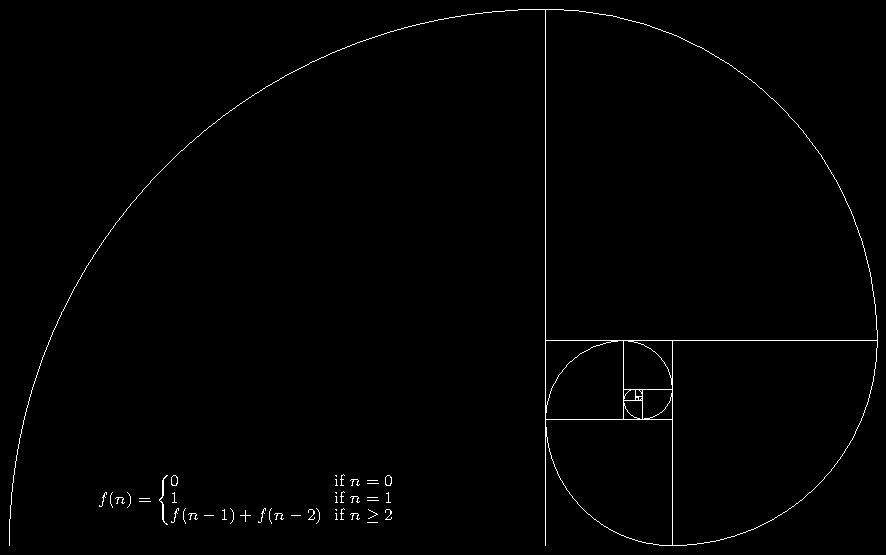
\includegraphics[width=2in]{fibonacci-spiral}\includegraphics[width=1in]{Rplot001}
\end{figure}



   \begin{center}

     {\bighelv ENG 2020 Intermediate Composition - Summer 2010} \\
     {\mediumhelv Science \& Technology Research} \\
     \ \\
     \ \\

     \begin{tabular}{ l r }

       \begin{tabular}{l}
          Instructor: Joshua Bowles      \\                                             
          Office: none                    \\                                                  
          E-mail: uvucompbowles@gmail.com  \\                                               
          Website: \href{http://sites.google.com/site/scitechcompositionandresearch/}{http://sites.google.com/site/scitechcompositionandresearch/}\\
          Blog: \href{http://linguisticlogic.wordpress.com/}{Linguistic Logic} 
\\ 
\\     
 \end{tabular}

       &

       \begin{tabular}{l}
          Class: MWF \\
          Office Hours: By appointment only \\ 
          \textbf{I do NOT use my UVU e-mail} \\                                                  
          %\phantom{Office Hours:} By appointment                \\                                               
                                            \\        
                                            \\                                     
       \end{tabular}

     \end{tabular}

   \end{center}
   \ \\


   {\bf Textbooks}\\
{\bf \textsl {A\&B}}: Ramage, John D., and John C. Bean, and June Johnson. {\sl The Allyn and Bacon Guide to 
Writing}. 5th edition. New York: Pearson Longman, 2009. ISBN-13:978-0-205-59873-1. 
(A link for used versions:  \href{http://www.amazon.com/Allyn-Bacon-Guide-Writing-MyCompLab/dp/0205598730/ref=sr
_1_3/175-1452668-8158623?ie=UTF8&s=books&qid=1245772101&sr=1-3}{here}.) \\
{\bf \textsl {DK}}: Wysocki, Anne Frances, and Dennis A. Lynch. {\sl The DK Handbook.} New York: Pearson Longman, 
2008. ISBN-13 978-0-321-42053-4. 
   \ \\

   {\bf Course Outline and Grades}\\
   We will focus on methods of analyzing ideas and how to communicate such methods (and their results) in written form. You will demonstrate your ability to think in written form (and your development) through the following:
   \begin{enumerate}
     \item Informative \& Surprising, 4-6 pgs
     \item Analysis \& Synthesis, 4-6 pgs
     \item Abstract \& Annotated Bibliography, 3 pgs
     \item Final: Classical Argument, 10-12 pgs
     \item A number of responses and one exam
   \end{enumerate}

The breakdown of grades and letter grade assignment will be according to the following:
\vskip 2mm
  
\begin{tabular}{|l|l|}
\hline
Attendance & 15\\
Responses/Exam & 15\\
3 Short Papers & 45\\
1 Final Paper & 20\\
Portfolio & 5\\
\hline
\end{tabular} \  \  \  \  \ \begin{tabular}{|l|l|}
   \hline
   93-100 gives A &  73-76 gives C\\
   90-92 gives A- & 70-72 gives C-\\
   87-89 gives B+ & 67-69 gives D+\\
   83-86 gives B & 63-66 gives D\\
   80-82 gives B- & 60-62 gives D-\\
   79-77 gives C+ & 00-59 gives E\\
   \hline 
   \end{tabular}
   \ \\
\newtheorem{comment}{Comment}
\begin{comment}
 Notice that I run an equivalent points = percentage scale: one point equals one percent. Keep this in mind when I say that something is worth $n$ points.
\end{comment}
 
\paragraph{The Focus of this class}   
is primarily on research that you will be directing yourself. This means that you need to develop a research agenda in conjunction with the course outline and goals. There is time given at the beginning of the semester to help you find an appropriate topic and develop a strategic course of action. Everything in this class is directed toward the final writing assignment: Paper 4, Classical Argument. This means you should think long-term about projects and you should begin doing research as early as you can.

\begin{comment}
You should find a research topic that engages you. Even things you think might not be ``allowed'' for a college paper (e.g., I have had students write about such varied things as time-travel, medieval knights, Mayan calender, alien life, et cetera). The point of attending University is to get the chance to have a \textbf{transformative experience}. You can have a good experience in this class, and do interesting research, if you pick topics that are really cool.
\end{comment}
\ \\
 {\bf Portfolio}\\
   Save {\bf ALL} written assignments in this class. I elaborate on this as the semester proceeds.
  \\ 

   {\bf Notes on the Calendar}\\
   \textcolor{red}{ATTENDANCE IS MANDATORY}. You are given an allowance of three full days. After that, each full day is worth $-2$ points. Also as the course proceeds we usually change the schedule. I say {\it we} because I take input from students seriously. However, if you miss class you miss the chance to help shape the class, and more importantly, you miss changes to the schedule. It is your responsibility to find out any information you miss.
   \\ 
       

   {\bf Academic Integrity}\\
 Cheating, plagiarism, or any unethical academic behavior is not tolerated. It will be reported immediately to 
your Major Department and Student Services. See plagiarism policy 
\href{http://www.uvu.edu/english/student/plagiarism.html}{here} or at http://www.uvu.edu/english/student/
plagiarism.html.
 \\

  
  {\bf Basic Resources}\\
  The following is a list (with active links) of some basic research corpora.
  \begin{enumerate}
\item UVU library: \href{http://www.uvu.edu/library}{http://www.uvu.edu/library}
\item Library search engines: \href{http://www.uvu.edu/library/search/index.php}{http://www.uvu.edu/library/search/index.php}
\item Useful databases: JSTOR, MEDLINE, especially ACADEMIC SEARCH PREMIER
\item Cornell science archive: \href{http://www.arXiv.org}{http://www.arXiv.org}
\item UVU writing center: \href{http://www.uvsc.edu/owl}{http://www.uvsc.edu/owl}
\end{enumerate}
\ \\
   %\vfill\eject
% 
\newpage
   {\bf  Schedule of Readings and Assignments}\\
   The schedule here is {\it tentative} and will most likely be modified. It is your responsibility to keep track of the changes as I announce them in class.
   \begin{enumerate}

\item (Week 1) May 5 W:  Introductions;  LECTURE/DISCUSSION: Syntax, Semantics, Pragmatics. \textbf{READ: A\&B pp. 212--219 \ \href{http://www.llc.ilstu.edu/dlevere/docs/currentanthroarticle.web.pdf}{Assigned I}}.
\item[] May 7 F: DISCUSSION: Assigned I. EXCERCISE: ``Walking Directions.'' LECTURE: Syntax, Semantics, Pragmatics. \textbf{READ: DK pp. 102-111}; \texttt{Start Paper 1}.

\item (Week 2) May 10 M: \texttt{RESPONSE TO ASSIGNED I DUE.} EXERCISE: ``Proof of Earth's Orbit.'' LECTURE: Evidence Types and (re-)Ranking. REVIEW: Thesis statement. \textbf{READ: A\&B pp. 221--225 \ \href{http://citeseerx.ist.psu.edu/viewdoc/summary?doi=10.1.1.55.8083}{Assigned II}}. 
\item[] May 12 W: DISCUSSION: Assigned II. LECTURE: What is Analysis and Rhetoric? REVIEW: Response to Assigned II.
\item[] May 14 F: \texttt{RESPONSE TO ASSIGNED II DUE.} REVIEW: Paper 1.
 
\item (Week 3) May 17 M: \textcolor{red}{\texttt{PAPER 1 DUE.}} \texttt{Start Paper 2}, \textbf{READ A\&B pp. 350--360 and 366--367}.
\item[] May 19 W: WRITING DAY (no class): work on your paper. 
\item[] May 21 F: LECTURE: Syntax, Semantics, Pragmatics. REVIEW: Paper 2. 

\item (Week 4)  May 24 M: \textcolor{red}{\texttt{PAPER 2 DUE.}} \texttt{Start Abstracts/Bibliographies}, \textbf{READ DK pp. 314--325} and skim over the rest of DK Part 8 (307--462).
\item[] May 26 W: LECTURE/REVIEW: Syntax, Semantics, Pragmatics. EXCERCISE: Presupposition. Second half: \textcolor{red}{Exam 1: Terminology and Concepts}.
\item[] May 28 F: RESEARCH DAY (no class): work on Bibliographies.

\item (Week--5) May 31 M: \textcolor{magenta}{HOLIDAY: Memorial Day}
\item[] June 2 W: \textcolor{red}{\texttt{ABSTRACT \& ANN. BIBLIOGRAPHY (\#3) DUE.}} \texttt{Start paper 4}. LECTURE: Syllogism \& Fallacy. RSRCH. PRESENTATIONS? 
\item[] June 4 F: RSRCH. PRESENTATIONS. Begin: \textbf{READ A\&B Chapters 14, 15}.

\item (Week 6) June 7 M: RSRCH. PRESENTATIONS 
\item[] June 9 W: RSRCH. PRESENTATIONS? 
\item[] June 11 F: REVIEW: Paper 4.

\item (Week 7) June 14 M: REVIEW: Paper 4.
\item[] June 16 W: REVIEW: Paper 4. (Earliest day to accept Portfolios)
\item[] June 18 F: Open discussion about Syntax, Semantics, Pragmatics.

\item (Week 8) June 21 M: \textcolor{red}{\texttt{PAPER 4 and PORTFOLIOS DUE}}
\item[] June 23 W: \textcolor{magenta}{END OF SEMESTER}
\end{enumerate}
% 
% 
% \section{Possible Research Topics}
% \begin{enumerate}
% \item Symmetry and Fibonacci patterns in nature and art
% \item Mathematics of probability (i.e., medicine, insurance, game shows, gambling, physics, marketing)
% \item Encryption and security
% \item Economics of personal and corporate debt
% \item Biology of stem cells, e.g., differentiation and reverse engineering\footnote{\emph{Many people} write papers on this topic.}
% \item Quantum computers, quantum computation, and the theory of quantum consciousness
% \item Science of alternative energy\footnote{Again, many people write on this subject.}
% \item Biographical life of a scientist---Newton, Einstein, Galileo, Galois, Abels, Cantor, Turing, Boole, Godel\ldots{}.
% \item Philosophy of science, religion, etc.\ldots
% \item Literature and consciousness
% \item Artificial Intelligence and Gaming
% \item Gaming and Social Networks
% \item Social Networking and `Hooking up'
% \item War
% \item Homosexuality: nature or nurture?
% \item Does racism exist? Is there a biological/evolutionary aspect to it?\end{enumerate}
% 
% \subsection{Comment}  
% You should find something that engages you. Even topics you think might not be ``allowed'' for a college paper (e.g., I have had students write about such varied things as time-travel, medieval knights, Mayan calender, alien life, \textsl{et cetera}). The point of attending University is to get the chance to have a \emph{transformative experience}. You can have a good experience in this class, and do interesting research, if you pick topics that are really cool.
% 
% \section{Citation formats, Organizations, Websites}
% \begin{itemize}
% \item \href{http://www.bedfordstmartins.com/online/citex.html}{Bedsford's St. Martins Press} MLA, APA, Chicago, and other styles 
% \item \href{http://www.library.cornell.edu/resrch/citmanage/mla}{Cornell University Library} MLA style guide
% \item \href{http://owl.english.purdue.edu/owl/resource/557/01/}{Purdue University Library} MLA style guide
% \item \href{http://owl.english.purdue.edu/owl/resource/560/01/}{Purdue University Library} APA style guide
% \item \href{http://www.lib.berkeley.edu/instruct/guides/mlastyle.pdf}{UC Berkeley Library} MLA style guide
% \item \href{http://languagelog.ldc.upenn.edu/nll/}{Modern Language Society (MLA)}
% \item\href{http://www.amwa.org/}{American Medical Writers Association}
% \item\href{http://www.attw.org/}{Association of Teachers of Technical Writing}
% \item\href{http://www.ieeepcs.org/}{IEEE Professional Communication Society}
% \item \href{http://standards.ieee.org/guides/style/2009_Style_Manual.pdf}{2009 IEEE Standards Style Manual}
% \item\href{http://nasw.org/}{National Association of Science Writers}
% \item\href{http://www.stc.org/}{Society for Technical Communication}\end{itemize}
% 
% \section{Research}
% \subsection{Databases}\begin{itemize}  
% \item Research tools accessible at the \href{http://www.uvu.edu/library/researchtools/index.html}{UVU-Library}
% \item \href{http://www.uvu.edu/library/guides/index.html}{Research guides} by topic at UVU library
% \item \href{http://www.uvu.edu/library/researchtools/electronic_encyclopedias.html}{Electronic Encyclopedias and Dictionaries}
% \item JSTOR 
% \item ScienceDirect 
% \item ERIC 
% \item Academic Search Premier 
% \item Project Muse
% \end{itemize}
% 
% \subsection{Other Links and Research Sources}
% \begin{itemize}
% \item \href{http://languagelog.ldc.upenn.edu/nll/}{Language Log}
% \item \href{http://mitpress.mit.edu}{MIT Press} 
% \item \href{http://arxiv.org}{Cornell ArXiv} 
% \item \href{http://plato.stanford.edu/}{Stanford Encyclopedia of Philosophy} 
% \item Academic web pages of \href{http://www.uvu.edu/profpages/profiles/show/user_id/530}{professors} for downloadable papers\footnote{Make sure these sites are connected to a University or College.}
% \end{itemize}

\end{document}

